\documentclass{beamer}
\usepackage[no-math]{fontspec}
\usepackage{xeCJK}
\setCJKmainfont{Source Han Sans TW}

\usetheme{CambridgeUS}
\title[ADHD]{Attention Deficit Hyperactivity Disorder}
\subtitle{Nelson 20th, Chapter 33}
\author[Chen-Pang He]{何震邦 (Chen-Pang He), M5 Clerk}
\date{May 25, 2017}

\institute[SKH \& TMU]
{
    Department of Pediatrics\\
    Shin Kong WHS Memorial Hospital
    \and
    School of Medicine\\
    Taipei Medical University
}

\begin{document}
\maketitle

\begin{frame}{Attention deficit hyperactivity disorder}
\begin{itemize}
    \item Most common neurobehavioral disorder of childhood
    \item Inattention
    \item Motor overactivity and restlessness
\end{itemize}
\end{frame}

\section{Etiology}
\begin{frame}{Etiology}
\begin{figure}
    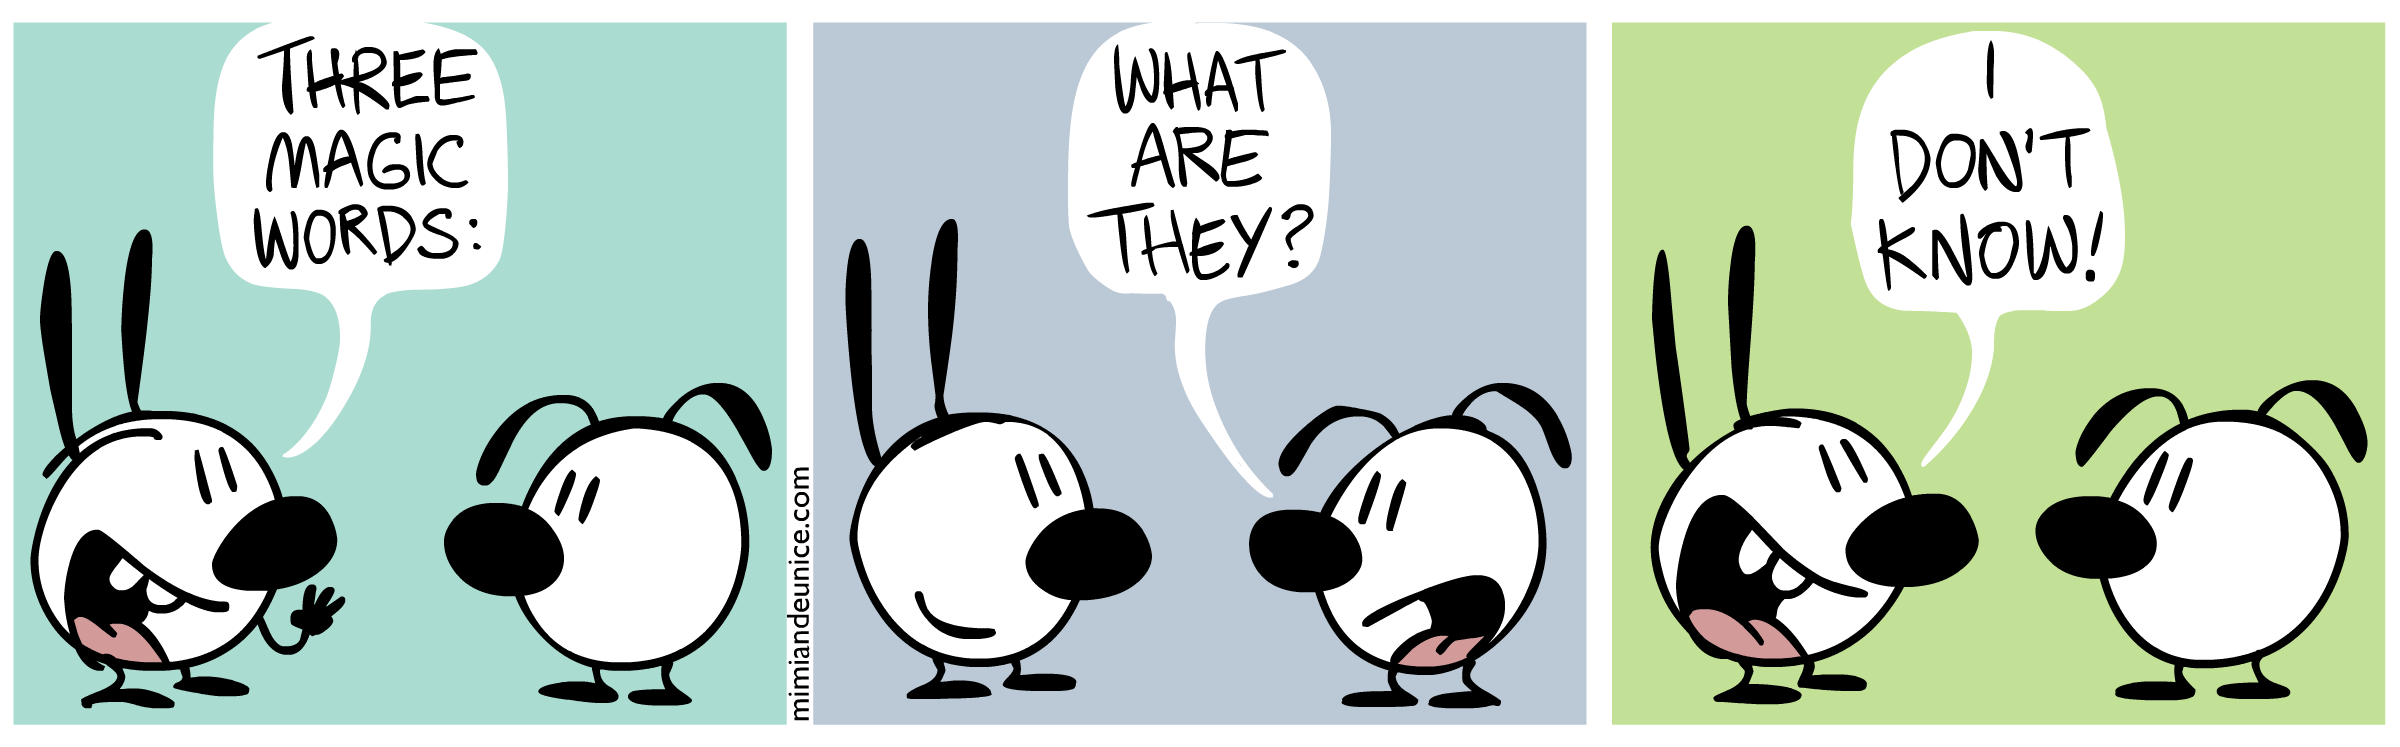
\includegraphics[width=\textwidth]{mimi-and-eunice.png}
    \caption{Mimi \& Eunice drawn by Nina Paley}
\end{figure}
\end{frame}

\begin{frame}{Unknown etiology}
\begin{quotation}
    I don't know -- but I'll do my best to find out for you.

    \begin{flushright}
        \upshape---Dr.~Stuart Foxman
    \end{flushright}
\end{quotation}
\end{frame}

\section{Epidemiology}
\begin{frame}{Global prevalence}
\begin{description}
    \item[School-aged] 9\%
    \item[Adolescents] 2--6\%
    \item[Adults] 2\%
\end{description}
\end{frame}

\begin{frame}{Epidemiology}
\begin{itemize}
    \item Underdiagnosis
    \item Undertreatment
    \item Comorbidity
    \begin{itemize}
        \item Opposition defiant disorder, conduct disorder, learning
            disabilities, depression, anxiety disorders, ...
    \end{itemize}

    \item Risk factors
    \begin{itemize}
        \item Epilepsies, neurofibromatosis, tuberous sclerosis
    \end{itemize}
\end{itemize}
\end{frame}

\section{Pathogenesis}
\begin{frame}{Pathogenesis}
MRI studies indicate

\begin{itemize}
    \item Loss of normal asymmetry in the brain
    \item Smaller volumes of specific structures
    \begin{itemize}
        \item Prefrontal cortex, basal ganglia, ...
        \item Rich in dopamine receptors
        \item 5--10\% reduction of volume
    \end{itemize}
\end{itemize}
\end{frame}

\begin{frame}{Functional MRI}
\begin{itemize}
    \item Low blood flow to the striatum
    \item Deficits in a widespread functional networks, including
    \begin{itemize}
        \item Striatum, prefrontal regions, parietal lobe, temporal lobe
    \end{itemize}
\end{itemize}
\end{frame}

\begin{frame}{Dopamine hypothesis}
Disturbances in the dopamine system may be related to the onset of ADHD.

\begin{itemize}
    \item Dopaminergic mechanisms of action of medication
    \item Identification of low levels of dopamine activity in adults
    \begin{itemize}
        \item Fluorodopa positron emission tomography
    \end{itemize}
\end{itemize}
\end{frame}

\section{Clinical manifestations}
\begin{frame}{Clinical manifestations}
\begin{itemize}
    \item Predominantly inattentive type
    \item Predominantly hyperactive--impulsive type
    \item Combined type
\end{itemize}
\end{frame}

\begin{frame}{Inattention}
\begin{enumerate}
    \item Often fails to give close attention to details or makes careless mistakes
    \item Often has difficulty sustaining attention in tasks or play activities
    \item Often does not seem to listen when spoken to directly
    \item Often does not follow through on instructions and fails to finish schoolwork, chores, or duties in the workplace
    \item Often has difficulty organizing tasks and activities
    \item Often avoids, dislikes, or is reluctant to engage in tasks that require sustained mental effort
    \item Often loses things necessary for tasks or activities
    \item Is often easily distracted by extraneous stimuli
    \item Is often forgetful in daily activities
\end{enumerate}
\end{frame}

\begin{frame}{Hyperactivity and impulsivity}
\begin{enumerate}
    \item Often fidgets with or taps hands or feet or squirms in seat
    \item Often leaves seat in situations when remaining seated is expected
    \item Often runs about or climbs in situations where it is inappropriate
    \item Often unable to play or engage in leisure activities quietly
    \item Is often ``on the go,'' acting as if ``driven by a motor''
    \item Often talks excessively
    \item Often blurts out an answer before a question has been completed
    \item Often has difficulty waiting his or her turn
    \item Often interrupts or intrudes on others
\end{enumerate}
\end{frame}

\section{Diagnosis and differential diagnosis}
\subsection{Diagnosis}
\begin{frame}{DSM-5 diagnostic criteria}
\begin{enumerate}
    \item \textbf{Inattention} or \textbf{hyperactivity and impulsitivity}
        \begin{itemize}
            \item 6 out of 9 symptoms
            \item Persisted for 6 months
            \item Inconsistent with developmental level
        \end{itemize}
    \item Some symptoms were present before 12
    \item Some symptoms are present in $>1$ setting
    \item Negative impact on QoL
    \item Rule out other psychoses and mental disorders
\end{enumerate}
\end{frame}

\begin{frame}{ICD-10 hyperkinetic disorder (HKD)}
Differences from DSM-5, U.S. criteria for ADHD or HKD

\begin{itemize}
    \item 6 out of 8 inattentive symptoms
    \item 3 out of 5 hyperactive symptoms
    \item 1 out of 4 impulsive symptoms
    \item Criteria met for $>1$ setting
\end{itemize}
\end{frame}

\begin{frame}{Behavior rating scales}
Behavior rating scales are useful in establishing the magnitude and
pervasiveness of the symptoms, but are not sufficient alone to make a
diagnosis of ADHD.
\end{frame}

\subsection{Differential diagnosis}
\begin{frame}{Differential diagnosis}
\begin{itemize}
    \item Psychosocial factors
    \item Diagnoses associated with ADHD behaviors
    \item Medical and neurological conditions
\end{itemize}
\end{frame}

\begin{frame}{Psychosocial factors}
\begin{itemize}
    \item Response to physical or sexual abuse
    \item Response to inappropriate parenting practices
    \item Response to parental psychopathology
    \item Response to acculturation
    \item Response to inappropriate classroom setting
\end{itemize}
\end{frame}

\begin{frame}{Diagnoses associated with ADHD behaviors}
\begin{itemize}
    \item Fragile X syndrome
    \item Fetal alcohol syndrome
    \item Pervasive developmental disorders
    \item Obsessive--compulsive disorder
    \item Gilles de la Tourette syndrome
    \item Attachment disorder with mixed emotions and conduct
\end{itemize}
\end{frame}

\begin{frame}{Medical and neurological conditions}
\begin{itemize}
    \item Thyroid disorders (including general resistance to thyroid hormone)
    \item Heavy metal poisoning (including lead)
    \item Adverse effects of medications
    \item Effects of abused substances
    \item Sensory deficits (hearing and vision)
    \item Auditory and visual processing disorders
    \item Neurodegenerative disorder, especially leukodystrophies
    \item Posttraumatic head injury
    \item Postencephalitic disorder
\end{itemize}
\end{frame}

\section{Treatment}
\begin{frame}{Treatment}
\begin{itemize}
    \item Psychosocial treatments
    \item Behaviorally oriented treatments
    \item Medications
\end{itemize}
\end{frame}

\subsection{Psychosocial treatments}
\begin{frame}{Psychosocial treatments}
\begin{enumerate}
    \item Discuss with the parents and child effects of ADHD
    \item Set goals for the family to improve the child's relationships, skills, and behaviors
    \item Introduce parent support groups with professional consultation
\end{enumerate}
\end{frame}

\subsection{Behaviorally oriented treatments}
\begin{frame}{Behaviorally oriented treatments}
\begin{enumerate}
    \item Identify targeted behaviors which impair the child's life
    \item Guide the parents and teachers to encourage desired behaviors.
\end{enumerate}

Behavioral treatments are particularly useful for children with complex
comorbidities and family stressors, when combined with medication.
\end{frame}

\section{Prognosis}
\begin{frame}{Prognosis}
Often persistent

\begin{itemize}
    \item 60--80\% from childhood to adolescence
    \item 60\% from adolescence to adulthood
\end{itemize}
\end{frame}

\section{Prevention}
\begin{frame}{Prevention}
Parent training for preschool youth with ADHD can reduce oppositional behavior.
\end{frame}
\end{document}
